\section{Results}\label{sec:results}
All values are test F1 (attack class, Eq.~\eqref{eq:metrics}), mean $\pm$ std over \nv{seeds} seeds (\nv{runs} runs); Table~\ref{tab:main}, Fig.~\ref{fig:bar}, paired tests in Table~\ref{tab:sig}.
\begin{table*}[t]
\centering
\caption{Test F1 (attack class), mean $\pm$ std over 10 seeds; best in bold. ``Senior'' fits preprocessing on all rows before the split; Central rows are not federated.}
\label{tab:main}
\tiny
\setlength{\tabcolsep}{2.4pt}
\begin{tabular}{lcccccc}
\toprule
Method & CIC IID & CIC Dir(1.0) & CIC Dir(0.3) & CIC Dir(0.1) & NBa Device & NBa IID \\
\midrule
Central SVM & 0.9960\,$\pm$\,0.0009 & 0.9960\,$\pm$\,0.0009 & 0.9960\,$\pm$\,0.0009 & 0.9960\,$\pm$\,0.0009 & 0.9168\,$\pm$\,0.1691 & 0.9169\,$\pm$\,0.1669 \\
Central RF & \textbf{0.9987\,$\pm$\,0.0002} & \textbf{0.9987\,$\pm$\,0.0003} & \textbf{0.9988\,$\pm$\,0.0002} & \textbf{0.9988\,$\pm$\,0.0002} & \textbf{0.9997\,$\pm$\,0.0003} & \textbf{0.9997\,$\pm$\,0.0003} \\
Senior (as released) & 0.9963\,$\pm$\,0.0008 & 0.9963\,$\pm$\,0.0008 & 0.9951\,$\pm$\,0.0010 & 0.9904\,$\pm$\,0.0035 & 0.8704\,$\pm$\,0.1660 & 0.8565\,$\pm$\,0.1881 \\
Senior (no leak) & 0.9962\,$\pm$\,0.0008 & 0.9958\,$\pm$\,0.0009 & 0.9952\,$\pm$\,0.0009 & 0.9892\,$\pm$\,0.0049 & 0.9226\,$\pm$\,0.1562 & 0.9252\,$\pm$\,0.1537 \\
Local-prep FedAvg & 0.9953\,$\pm$\,0.0010 & 0.9388\,$\pm$\,0.0330 & 0.7663\,$\pm$\,0.1181 & 0.5754\,$\pm$\,0.1963 & 0.6231\,$\pm$\,0.0905 & 0.9987\,$\pm$\,0.0002 \\
FedStat-FS (proposed) & 0.9946\,$\pm$\,0.0029 & 0.9942\,$\pm$\,0.0026 & 0.9918\,$\pm$\,0.0037 & 0.9913\,$\pm$\,0.0035 & 0.9264\,$\pm$\,0.1505 & 0.9065\,$\pm$\,0.1928 \\
FedStat-FS + FedProx & 0.9904\,$\pm$\,0.0044 & 0.9897\,$\pm$\,0.0035 & 0.9890\,$\pm$\,0.0028 & 0.9895\,$\pm$\,0.0032 & 0.9263\,$\pm$\,0.1506 & 0.9282\,$\pm$\,0.1468 \\
FedAvg-MLP (fed. prep) & 0.9961\,$\pm$\,0.0009 & 0.9962\,$\pm$\,0.0010 & 0.9961\,$\pm$\,0.0009 & 0.9959\,$\pm$\,0.0009 & 0.9730\,$\pm$\,0.0509 & 0.9806\,$\pm$\,0.0359 \\
\bottomrule
\end{tabular}
\end{table*}
\begin{figure*}[t]
\centering
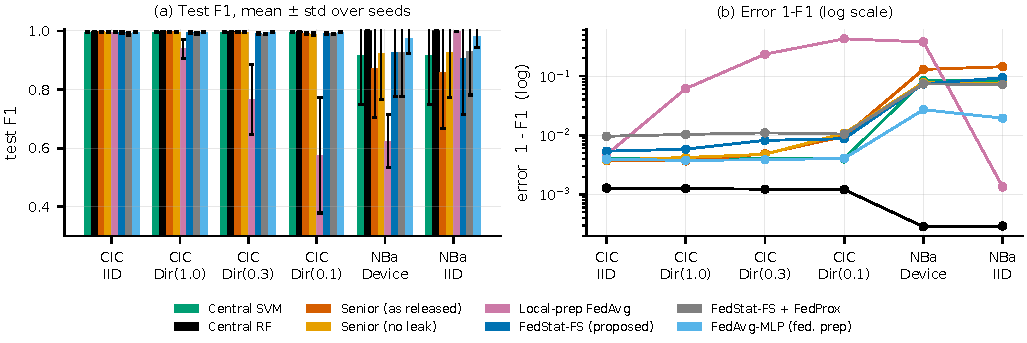
\includegraphics[width=0.78\textwidth]{fig_bar_f1.pdf}
\caption{Test F1 of all methods under every client regime (a) and the same means as error $1-F_1$ on a log scale (b). Error bars: std over seeds. NBa = N-BaIoT.}
\label{fig:bar}
\end{figure*}

\textbf{RQ1: fidelity and leakage.} In all \nv{exact_ok} of \nv{exact_total} FedStat-FS runs the subset computed from client statistics was identical to the pooled training-only subset (Jaccard \nv{exact_minjac}), and equal to that of \emph{Senior (no leak)} in \nv{same_as_pooled_ok}/\nv{same_as_pooled_total} paired comparisons: the federated preprocessing is exact, also under the strongest skew. Fitting preprocessing on all rows (Senior) instead of training rows changed CIC-IoT2023 F1 by \sg{senior}{senior_noleak}{ciciot}{iid}{diff} at IID ($p=$ \sg{senior}{senior_noleak}{ciciot}{iid}{pw}) and \sg{senior}{senior_noleak}{ciciot}{dir0.1}{diff} at Dir(0.1) ($p=$ \sg{senior}{senior_noleak}{ciciot}{dir0.1}{pw}); on N-BaIoT the leaky variant is \emph{worse} (\sg{senior}{senior_noleak}{nbaiot}{device}{diff}), plausibly because pooling all rows changes the selected subset. \emph{Answer: exact, and no measurable leakage optimism here (the pooled protocol stays privacy-inconsistent regardless).}

\textbf{RQ2: heterogeneity.} Under IID clients all federated pipelines coincide (CIC-IoT2023: Local-prep \rv{local_prep_fedavg}{ciciot}{iid}{f1m}, FedStat-FS \rv{fedstat}{ciciot}{iid}{f1m}). As skew grows, naive local preprocessing degrades to \rv{local_prep_fedavg}{ciciot}{dir1.0}{f1m}, \rv{local_prep_fedavg}{ciciot}{dir0.3}{f1m} and \rv{local_prep_fedavg}{ciciot}{dir0.1}{f1m} at Dir(1.0/0.3/0.1) (F1 $<0.9$ in \rv{local_prep_fedavg}{ciciot}{dir0.1}{nfail} of \rv{local_prep_fedavg}{ciciot}{dir0.1}{nruns} Dir(0.1) runs), whereas FedStat-FS holds \rv{fedstat}{ciciot}{dir1.0}{f1m}, \rv{fedstat}{ciciot}{dir0.3}{f1m} and \rv{fedstat}{ciciot}{dir0.1}{f1m}; on the natural per-device federation the gap is \rv{local_prep_fedavg}{nbaiot}{device}{f1m} versus \rv{fedstat}{nbaiot}{device}{f1m}. At Dir(0.1), $\Delta F_1=$ \sg{fedstat}{local_prep_fedavg}{ciciot}{dir0.1}{diff} (95\% CI [\sg{fedstat}{local_prep_fedavg}{ciciot}{dir0.1}{cilo}, \sg{fedstat}{local_prep_fedavg}{ciciot}{dir0.1}{cihi}]; raw $p=$ \sg{fedstat}{local_prep_fedavg}{ciciot}{dir0.1}{pw}, the floor for \nv{seeds} seeds, so every seed favours FedStat-FS; Holm over all tests \sg{fedstat}{local_prep_fedavg}{ciciot}{dir0.1}{pwholm}; post hoc, Holm within this comparison's six regimes \sg{fedstat}{local_prep_fedavg}{ciciot}{dir0.1}{pwholmpair}): large and consistent, but significant only under the less conservative family.

The ablations (Table~\ref{tab:ablation}, Fig.~\ref{fig:abl}) locate the cause. Federated selection with per-client \emph{scaling} (A1) is even worse than Local-prep (Dir(0.1): \rv{abl_localscale}{ciciot}{dir0.1}{f1m}): clients with different traffic mixes learn weights in different coordinate systems that cannot be averaged. Local voting also selects other features (Jaccard \nv{jaclocal:ciciot:iid} at IID, \nv{jaclocal:ciciot:dir0.1} at Dir(0.1), \nv{jaclocal:nbaiot:device} on devices; Fig.~\ref{fig:sel}). One-shot cold-start averaging (A3) costs $\Delta F_1=$ \sg{fedstat}{abl_oneshot}{ciciot}{dir0.1}{diff} at Dir(0.1) (raw $p=$ \sg{fedstat}{abl_oneshot}{ciciot}{dir0.1}{pw}, Holm \sg{fedstat}{abl_oneshot}{ciciot}{dir0.1}{pwholm}), a mild trend only. \emph{Answer: a common standardiser from shared statistics is what keeps a federated linear detector usable under non-IID clients.}
\begin{table*}[t]
\centering
\caption{Ablations (test F1, mean $\pm$ std): A1 per-client scalers; A2 no selection; A3 one-shot averaging; A4 Pearson-only / LDA-only. A1 and A3 inherit the tuned FedStat-FS hyper-parameters; A2 and A4 are tuned separately.}
\label{tab:ablation}
\tiny
\setlength{\tabcolsep}{2.4pt}
\begin{tabular}{lccccccc}
\toprule
Method & CIC IID & CIC Dir(1.0) & CIC Dir(0.3) & CIC Dir(0.1) & NBa Device & NBa IID & \#feat (CIC / NBa) \\
\midrule
FedStat-FS (proposed) & 0.9946\,$\pm$\,0.0029 & 0.9942\,$\pm$\,0.0026 & 0.9918\,$\pm$\,0.0037 & 0.9913\,$\pm$\,0.0035 & 0.9264\,$\pm$\,0.1505 & 0.9065\,$\pm$\,0.1928 & 16 / 16 \\
A1: local scalers & 0.9946\,$\pm$\,0.0029 & 0.9189\,$\pm$\,0.0490 & 0.6417\,$\pm$\,0.0927 & 0.3552\,$\pm$\,0.2722 & 0.9514\,$\pm$\,0.0965 & 0.9080\,$\pm$\,0.1897 & 16 / 16 \\
A2: no selection & \textbf{0.9969\,$\pm$\,0.0002} & \textbf{0.9971\,$\pm$\,0.0003} & 0.9954\,$\pm$\,0.0016 & 0.9934\,$\pm$\,0.0022 & \textbf{0.9997\,$\pm$\,0.0001} & \textbf{0.9997\,$\pm$\,0.0001} & 34 / 111 \\
A3: one-shot averaging & 0.9943\,$\pm$\,0.0038 & 0.9927\,$\pm$\,0.0075 & 0.9934\,$\pm$\,0.0027 & 0.9806\,$\pm$\,0.0201 & 0.9569\,$\pm$\,0.0834 & 0.9087\,$\pm$\,0.1880 & 16 / 16 \\
A4a: Pearson only & 0.9967\,$\pm$\,0.0005 & 0.9968\,$\pm$\,0.0004 & \textbf{0.9965\,$\pm$\,0.0010} & \textbf{0.9936\,$\pm$\,0.0037} & 0.9993\,$\pm$\,0.0002 & 0.9995\,$\pm$\,0.0001 & 23 / 59 \\
A4b: LDA only & 0.9965\,$\pm$\,0.0003 & 0.9955\,$\pm$\,0.0014 & 0.9946\,$\pm$\,0.0013 & \textbf{0.9936\,$\pm$\,0.0020} & 0.9283\,$\pm$\,0.1464 & 0.9103\,$\pm$\,0.1851 & 20 / 20 \\
\bottomrule
\end{tabular}
\end{table*}
\begin{figure*}[t]
\centering
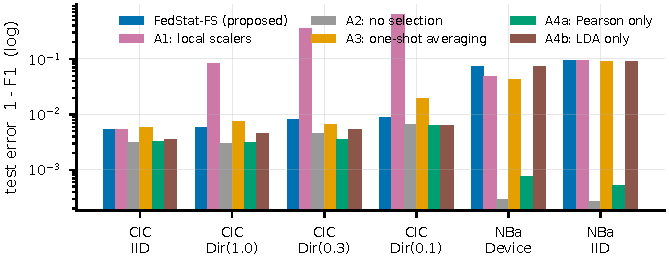
\includegraphics[width=0.64\textwidth]{fig_ablation.pdf}\hfill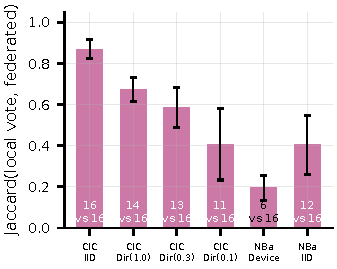
\includegraphics[width=0.34\textwidth]{fig_selection.pdf}
\caption{Left: ablation of the new components as test error $1-F_1$ (log scale; A1 per-client scalers, A2 no selection, A3 one-shot averaging, A4 Pearson-only / LDA-only). Right: agreement (Jaccard) between the locally voted and the federated feature subsets; numbers in bars: subset sizes (local vs federated).}
\label{fig:abl}\label{fig:sel}
\end{figure*}

\textbf{Selection is not the beneficial part.} The Pearson--LDA intersection did not improve accuracy. On CIC-IoT2023, no selection (\nv{nfeat:nosel:ciciot} features) and Pearson-only reach \rv{abl_nosel}{ciciot}{iid}{f1m} and \rv{abl_pearson}{ciciot}{iid}{f1m} at IID versus \rv{fedstat}{ciciot}{iid}{f1m} for the \nv{nfeat:fedstat:ciciot}-feature intersection ($\Delta F_1=$ \sg{fedstat}{abl_nosel}{ciciot}{iid}{diff}, raw $p=$ \sg{fedstat}{abl_nosel}{ciciot}{iid}{pw}, Holm \sg{fedstat}{abl_nosel}{ciciot}{iid}{pwholm}): compression halves the input at a small accuracy price. On N-BaIoT it is \emph{unstable}: every linear model that uses it fails (F1 $<0.9$) on the same seeds (FedStat-FS \nv{nfail:fedstat:nbaiot}/\nv{nrun:fedstat:nbaiot} runs, Central SVM \nv{nfail:central_svm:nbaiot}, Senior no leak \nv{nfail:senior_noleak:nbaiot}; Senior, whose all-row fit picks other subsets, \nv{nfail:senior:nbaiot}), while Pearson-only, no selection and the random forest never fail (\nv{nfail:abl_pearson:nbaiot}, \nv{nfail:abl_nosel:nbaiot}). This is a property of the rule, not of federation: exact solvers on the pooled \emph{training} split reach F1 \nv{diag:6:intersection:trainf1} with the \nv{diag:6:intersection:nfeat}-feature subset of a failing seed, versus \nv{diag:6:pearson:testf1} with Pearson-only and \nv{diag:6:none:testf1} with all features.
\textbf{RQ3: cost and competitiveness.} The linear detector has \nv{cost:fedstat:params} parameters, trains in \nv{cost:fedstat:train}\,s and classifies 1000 flows in \nv{cost:fedstat:infer}\,ms, against \nv{cost:fedstat_mlp:params} parameters, \nv{cost:fedstat_mlp:train}\,s and \nv{cost:fedstat_mlp:infer}\,ms for the federated MLP (Table~\ref{tab:cost}). The one-off statistics upload is \nv{statbytes:cic}\,KB per client for 46 features (\nv{statbytes:nba}\,KB for 115): more than the \emph{whole} model traffic of the linear detector (\nv{modelKB:cic}\,KB over all rounds and clients) but far below the MLP's. FedStat-FS is slightly below the centralised SVM ($\Delta F_1=$ \sg{fedstat}{central_svm}{ciciot}{iid}{diff} at CIC IID, raw $p=$ \sg{fedstat}{central_svm}{ciciot}{iid}{pw}, Holm \sg{fedstat}{central_svm}{ciciot}{iid}{pwholm}); the federated MLP matches it (\rv{fedstat_mlp}{ciciot}{iid}{f1m}) and the pooled forest is the ceiling (\rv{central_rf}{ciciot}{iid}{f1m}). FedProx did not help (\rv{fedstat_prox}{ciciot}{dir0.1}{f1m} against \rv{fedstat}{ciciot}{dir0.1}{f1m} at Dir(0.1)), as expected when drift comes from scaling. \emph{Answer: the extra communication is small and one-off; the linear detector classifies two to three orders of magnitude faster than the MLP or forest, at \nv{mlpgap:min}--\nv{mlpgap:max} F1 points below the MLP on CIC-IoT2023.}
\begin{table*}[t]
\centering
\caption{Computational cost on CPU (CIC-IoT2023, seed 0, IID clients; whole simulated federation on one machine; cold run in a fresh process, median of three; the RAM column is noisy, roughly $\pm$100 MB, and dominated by data copies). Traffic counts float32 model up/down-loads over all rounds; the statistics upload is float64, once.}
\label{tab:cost}
\tiny
\setlength{\tabcolsep}{2.4pt}
\begin{tabular}{lccccccc}
\toprule
Method & Train (s) & Preproc. (s) & Inference (ms/1k flows) & Parameters & Peak extra RAM (MB) & Model traffic (KB, whole run) & Stats upload (KB/client) \\
\midrule
Central SVM & 2.1 & 0.11 & 0.01 & 17 & 176 & 0.0 & 0 \\
Central RF & 2.3 & 0.14 & 3.87 & 28,880 & 175 & 0.0 & 0 \\
Senior (as released) & 0.5 & 0.23 & 0.01 & 17 & 296 & 2.0 & 0 \\
FedStat-FS (proposed) & 4.8 & 0.10 & 0.01 & 17 & 175 & 26.6 & 33.8 \\
FedStat-FS + FedProx & 4.8 & 0.13 & 0.01 & 17 & 85 & 26.6 & 33.8 \\
FedAvg-MLP (fed. prep) & 31.3 & 0.09 & 16.38 & 6,801 & 122 & 10626.6 & 33.8 \\
\bottomrule
\end{tabular}
\end{table*}

\textbf{Training, sensitivity and errors.} Fig.~\ref{fig:curves} shows convergence within a few rounds under IID and device clients and more slowly under Dir(0.1) (validation loss still falling at round 20; the local training loss rises as local models stop over-fitting their own classes). In the sensitivity study (validation, CIC Dir(0.3), Fig.~\ref{fig:sens}) FedStat-FS varies between \nv{sens:fedstat:tau:min} and \nv{sens:fedstat:tau:max} over $\tau$ (best at $\tau=0.1$: more features), rises with the LDA budget from \nv{sens:fedstat:lda_top:min} to \nv{sens:fedstat:lda_top:max} and is flat in rounds; no setting rescues Local-prep (best \nv{sens:local_prep_fedavg:lda_top:max}). Errors (Fig.~\ref{fig:err}, \ref{fig:cm}) concentrate in the rarest classes: SlowLoris and HTTP flood are missed by all four methods including the forest, fragmentation floods are also hard for linear detectors, and Local-prep additionally misclassifies the large flood classes and, on N-BaIoT, confuses junk and combo floods with benign traffic.
\begin{figure*}[t]
\centering
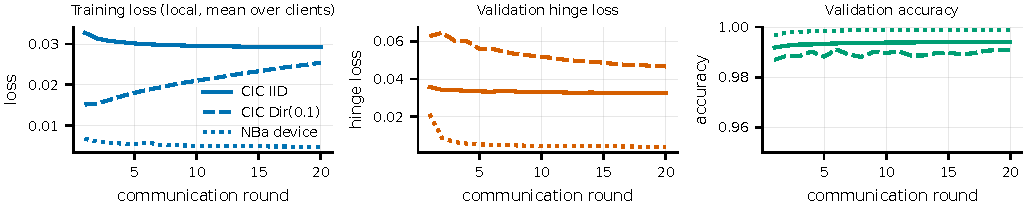
\includegraphics[width=0.78\textwidth]{fig_curves.pdf}\\[2pt]
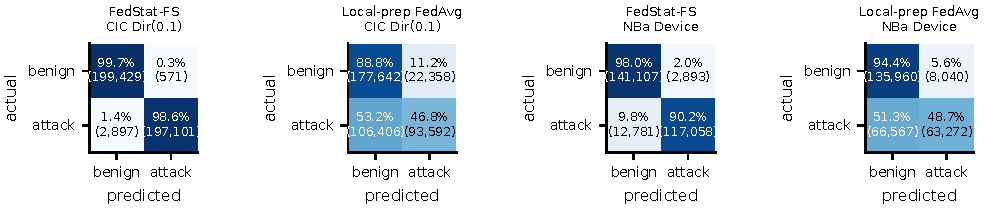
\includegraphics[width=0.78\textwidth]{fig_confusion.pdf}
\caption{Top: convergence of FedStat-FS (seed 0): local training loss, validation hinge loss and validation accuracy per round. Bottom: confusion matrices (summed over seeds, row-normalised, counts in brackets) for FedStat-FS and Local-prep FedAvg under CIC Dir(0.1) and N-BaIoT device clients.}
\label{fig:curves}\label{fig:cm}
\end{figure*}
\begin{figure*}[t]
\centering
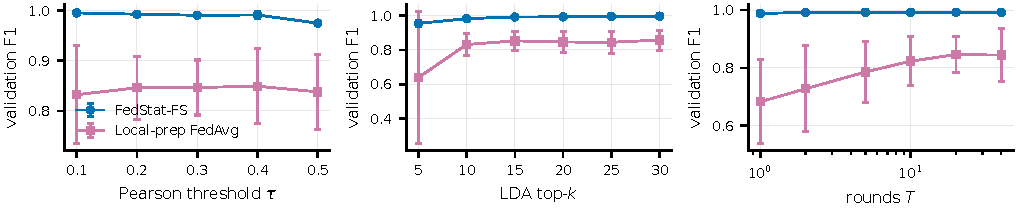
\includegraphics[width=0.78\textwidth]{fig_sensitivity.pdf}\\[2pt]
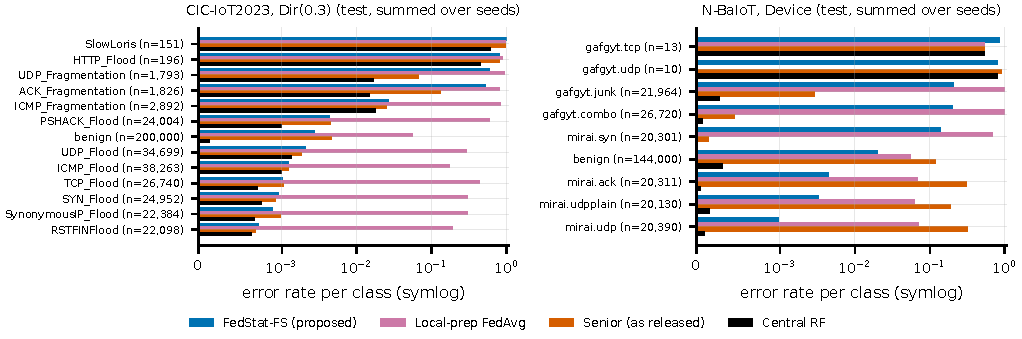
\includegraphics[width=0.78\textwidth]{fig_error.pdf}
\caption{Top: validation F1 versus Pearson threshold $\tau$, LDA top-$k_L$ and rounds $T$ (CIC Dir(0.3), 5 seeds). Bottom: per-class test error rate (symlog axis), summed over seeds, with class sizes.}
\label{fig:sens}\label{fig:err}
\end{figure*}
\begin{table*}[t]
\centering
\caption{Paired tests over 10 seeds (test F1): $\Delta$F1 = A $-$ B; $p$ = Wilcoxon signed-rank, raw / Holm over all 54 tests (full list with intervals in the CSV; smallest attainable $p$ = 0.0020).}
\label{tab:sig}
\tiny
\setlength{\tabcolsep}{2.4pt}
\begin{tabular}{lcccccc}
\toprule
Comparison (A vs B) & CIC IID: $\Delta$F1 & CIC IID: $p$ / Holm & CIC Dir(0.1): $\Delta$F1 & CIC Dir(0.1): $p$ / Holm & N-B Device: $\Delta$F1 & N-B Device: $p$ / Holm \\
\midrule
Senior (as released) vs Senior (no leak) & +0.0001 & 0.461/1.000 & +0.0012 & 0.375/1.000 & -0.0522 & 0.625/1.000 \\
FedStat-FS (proposed) vs Local-prep FedAvg & -0.0007 & 0.695/1.000 & +0.4159 & 0.002/0.105 & +0.3032 & 0.010/0.312 \\
FedStat-FS (proposed) vs A2: no selection & -0.0023 & 0.002/0.105 & -0.0021 & 0.049/1.000 & -0.0733 & 0.002/0.105 \\
FedStat-FS (proposed) vs A3: one-shot averaging & +0.0004 & 0.625/1.000 & +0.0107 & 0.027/0.820 & -0.0305 & 0.432/1.000 \\
FedStat-FS (proposed) vs Central SVM & -0.0014 & 0.002/0.105 & -0.0047 & 0.002/0.105 & +0.0095 & 1.000/1.000 \\
FedStat-FS (proposed) vs Senior (as released) & -0.0017 & 0.002/0.105 & +0.0008 & 0.432/1.000 & +0.0560 & 1.000/1.000 \\
FedStat-FS (proposed) vs FedAvg-MLP (fed. prep) & -0.0014 & 0.002/0.105 & -0.0047 & 0.004/0.141 & -0.0466 & 0.432/1.000 \\
\bottomrule
\end{tabular}
\end{table*}
